\documentclass{article}
%\usepackage{geometry}
%\geometry{top = 1in, bottom = 1in, left = 1in, right = 1in}
\usepackage[top = 0.7in, bottom = 0.7in, left = 0.7in, right = 0.7in]{geometry}
\usepackage{amsmath,amssymb,amsthm,mathrsfs}
\usepackage{graphicx}
\usepackage{bm}
\usepackage{float}
\usepackage[font=footnotesize,labelfont=bf]{caption}
\usepackage{movie15}
\usepackage{hyperref}

\usepackage{fancyhdr}
\pagestyle{fancy}
\rhead{\footnotesize {09/05/2012 ; MESA version 4442} }
\chead{\footnotesize {Authors: Jared Brooks, Lars Bildsten, Bill Paxton} }
\lhead{\footnotesize {mesa/star/test\_suite/7M\_prems\_to\_AGB} }

\begin{document}
	
	\begin{center}
	  \begin{Large}
	    \textbf{7M PREMS TO AGB}\\
	  \end{Large}
	\end{center}

        This test is to show a 7 $M_\odot$ pre-main sequence star evolved to the Asymptotic Giant Branch.  Therefore, this test should be cut off when the log of the surface luminosity reaches 4.3 (\texttt{log\_L\_upper\_limit = 4.3}).\\

        The inlist for this test sets the nuclear reaction network (\texttt{new\_net\_name = 'o18\_and\_ne22.net'}), the atmosphere option (\texttt{which\_atm\_option = 'simple\_photosphere'}, and some overshooting, mass loss, and opacity controls.\\

        The HR-diagram below shows the evolution through the whole run (figure \ref{fig:1}), with some important transitions marked by the colored dots.  The red dot marks the start of the main sequence.  The blue dot marks the end of hydrogen burning in the core.  The green dot marks the start of helium burning in the core.  The orange dot marks the end of helium burning in the core.  After the orange dot, helium and hydrogen burning continue in hot shells around the core until the maximum luminosity is reached

        \begin{figure}[H]
          \centering
          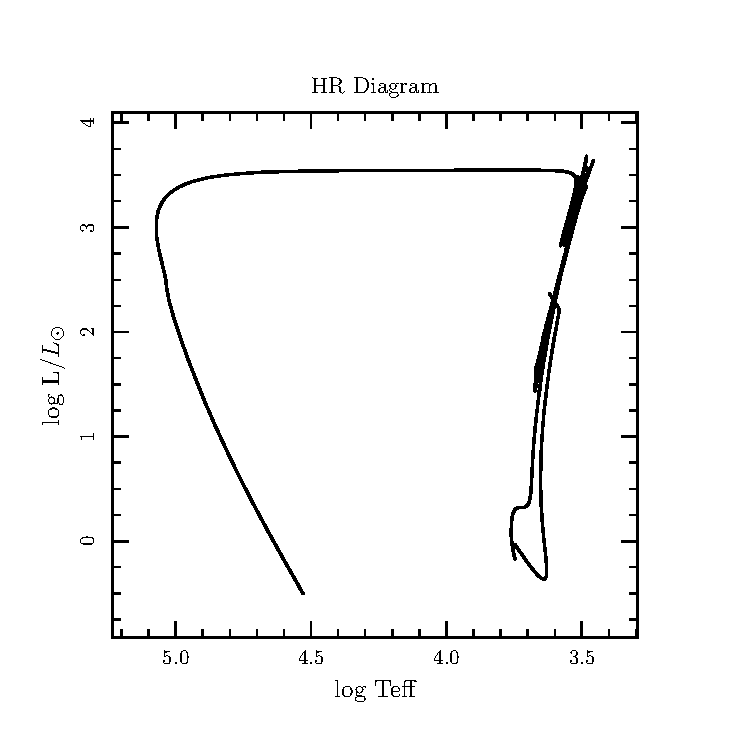
\includegraphics[width = 5in]{/Users/jaredbrooks/7M_prems_to_AGB/plots_out/HR_Diagram.pdf}
          \caption{Red: start of pre ms, Blue: end of H burning in core, Green: start of He burning in core, Orange: end of He burning in core}
          \label{fig:1}
        \end{figure}

        \pagebreak

        Below are an abundance profile (figure \ref{fig:2}) and a burning rate profile (figure \ref{fig:3}) from the start of the main sequence (red dot on HR-diagram, figure \ref{fig:1})

        \begin{figure}[H]
          \begin{minipage}[b]{0.5\linewidth}
	    \centering
	    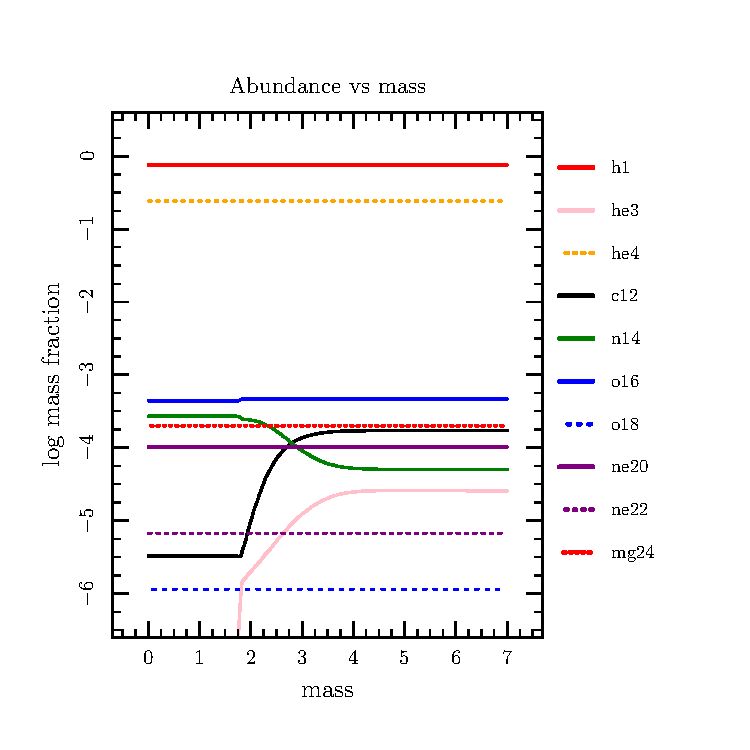
\includegraphics[width = 3.8in]{/Users/jaredbrooks/7M_prems_to_AGB/plots_out/Abundance_vs_mass_20.pdf}
	    \caption{Abundance profile at red dot}
	    \label{fig:2}
          \end{minipage}
          \hspace{0cm}
          \begin{minipage}[b]{0.5\linewidth}
            \centering
            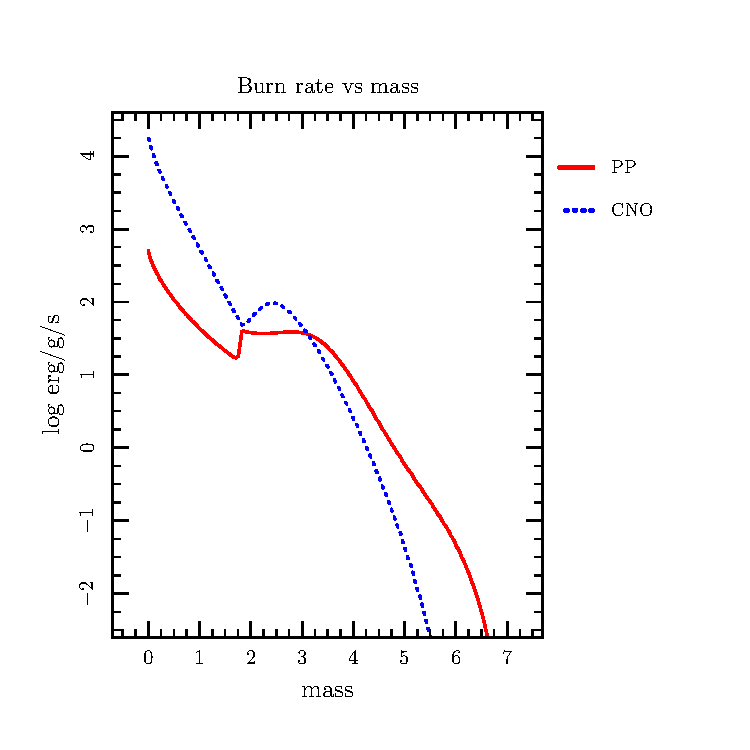
\includegraphics[width = 3.8in]{/Users/jaredbrooks/7M_prems_to_AGB/plots_out/Burnrate_vs_mass_20.pdf}
            \caption{Burning rate profile at red dot}
            \label{fig:3}
          \end{minipage}
	\end{figure}

        Below are an abundance profile (figure \ref{fig:4}) and a burning rate profile (figure \ref{fig:5}) from the end of hydrogen burning in the core (blue dot on HR-diagram,figure \ref{fig:1})

        \begin{figure}[H]
            \begin{minipage}[b]{0.5\linewidth}
            \centering
            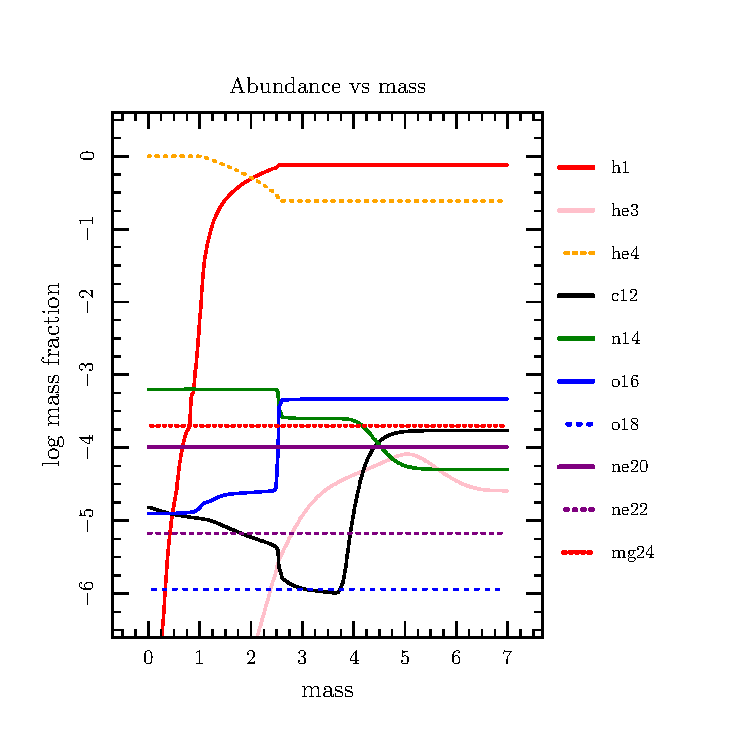
\includegraphics[width = 3.8in]{/Users/jaredbrooks/7M_prems_to_AGB/plots_out/Abundance_vs_mass_28.pdf}
            \caption{Abundance profile at blue dot}
            \label{fig:4}
          \end{minipage}
          \hspace{0cm}
          \begin{minipage}[b]{0.5\linewidth}
            \centering
            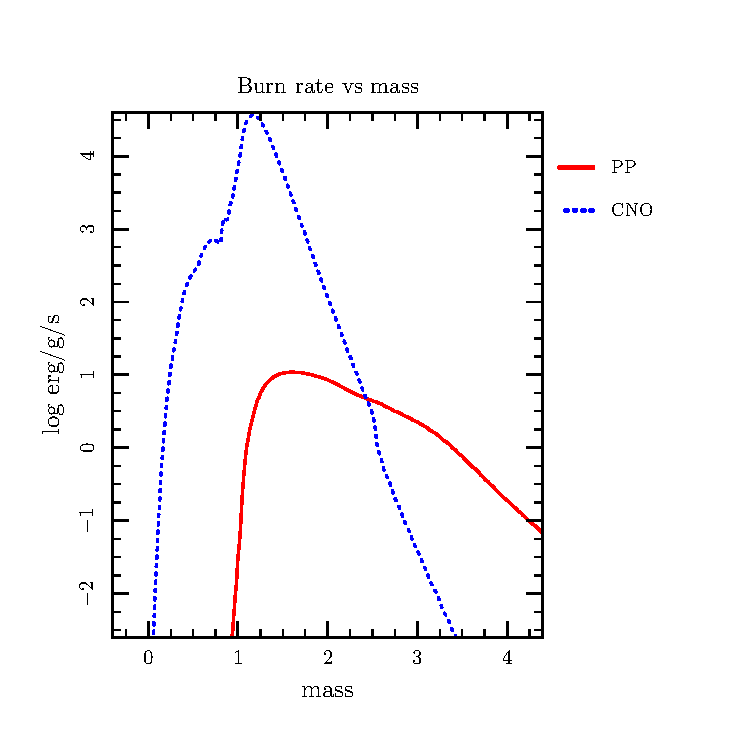
\includegraphics[width = 3.8in]{/Users/jaredbrooks/7M_prems_to_AGB/plots_out/Burnrate_vs_mass_28.pdf}
            \caption{Burning rate profile at blue dot}
            \label{fig:5}
          \end{minipage}
        \end{figure}

        \pagebreak

        Below are an abundance profile (figure \ref{fig:6}) and a burning rate profile (figure \ref{fig:7}) from the start of helium burning in the core (green dot on HR-diagram,figure \ref{fig:1})

        \begin{figure}[H]
          \begin{minipage}[b]{0.5\linewidth}
            \centering
            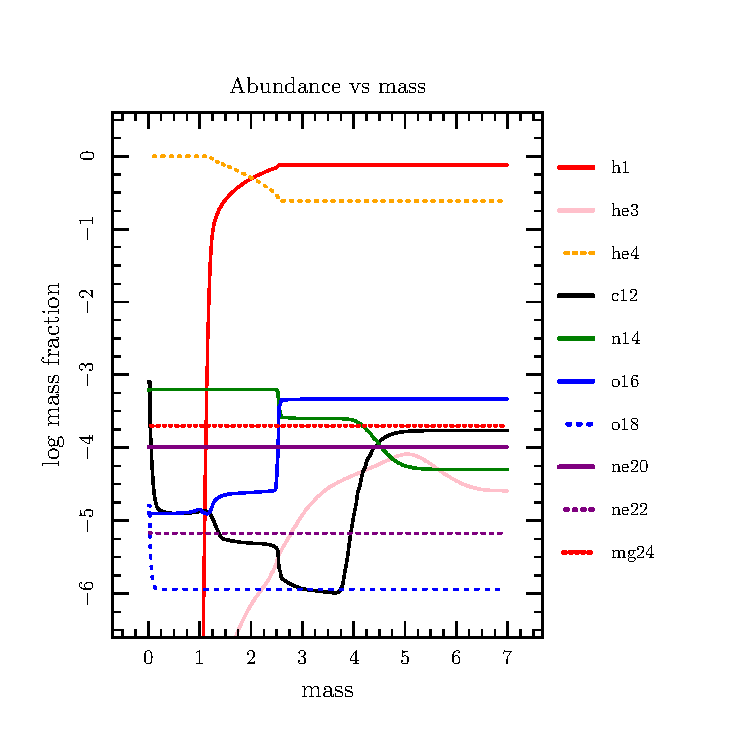
\includegraphics[width = 3.8in]{/Users/jaredbrooks/7M_prems_to_AGB/plots_out/Abundance_vs_mass_34.pdf}
            \caption{Abundance profile at green dot}
            \label{fig:6}
          \end{minipage}
          \hspace{0cm}
          \begin{minipage}[b]{0.5\linewidth}
            \centering
            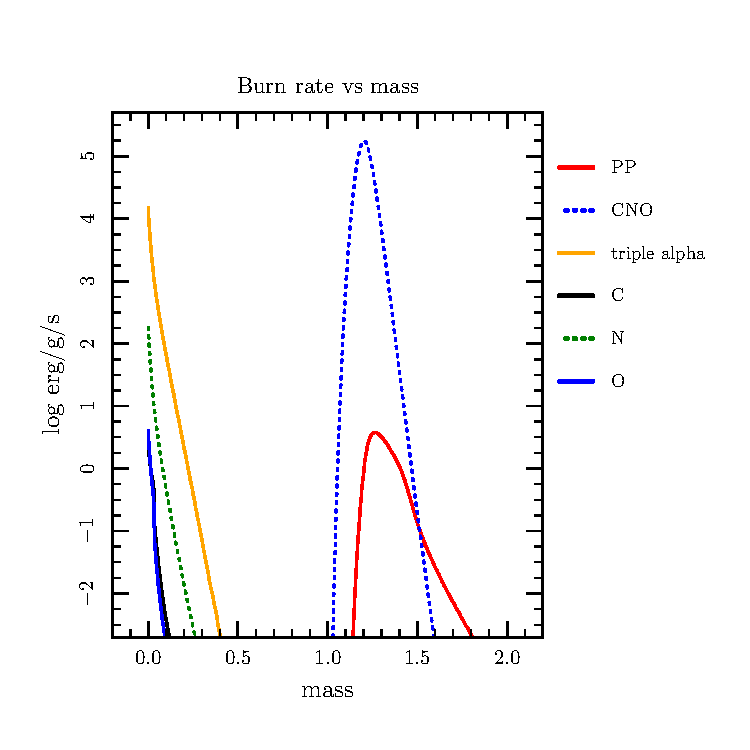
\includegraphics[width = 3.8in]{/Users/jaredbrooks/7M_prems_to_AGB/plots_out/Burnrate_vs_mass_34.pdf}
            \caption{Burning rate profile at green dot}
            \label{fig:7}
          \end{minipage}
        \end{figure}

        Below are an abundance profile (figure \ref{fig:8}) and a burning rate profile (figure \ref{fig:9}) from the end of helium burning in the core (orange dot on HR-diagram, figure \ref{fig:1})

        \begin{figure}[H]
          \begin{minipage}[b]{0.5\linewidth}
            \centering
            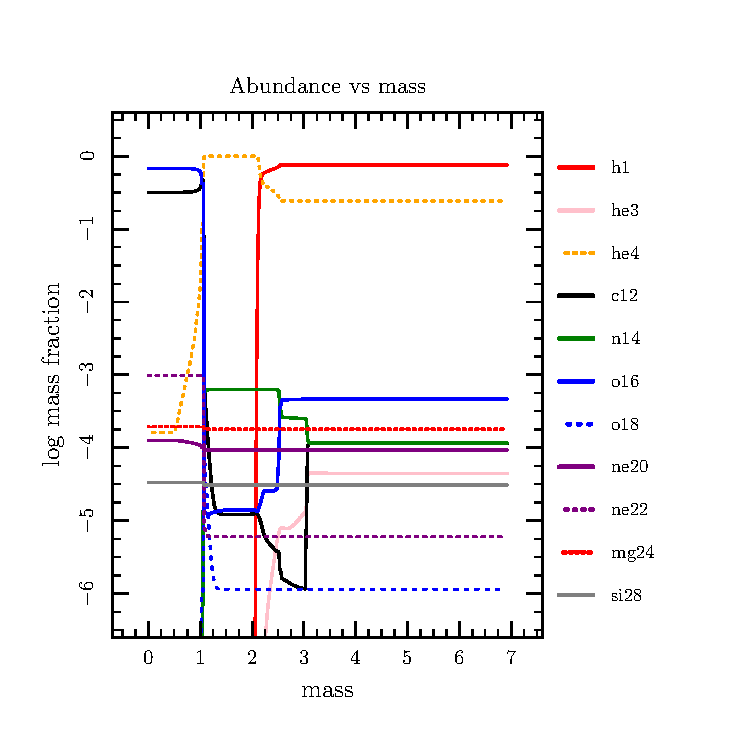
\includegraphics[width = 3.8in]{/Users/jaredbrooks/7M_prems_to_AGB/plots_out/Abundance_vs_mass_52.pdf}
            \caption{Abundance profile at orange dot}
            \label{fig:8}
          \end{minipage}
          \hspace{0cm}
          \begin{minipage}[b]{0.5\linewidth}
            \centering
            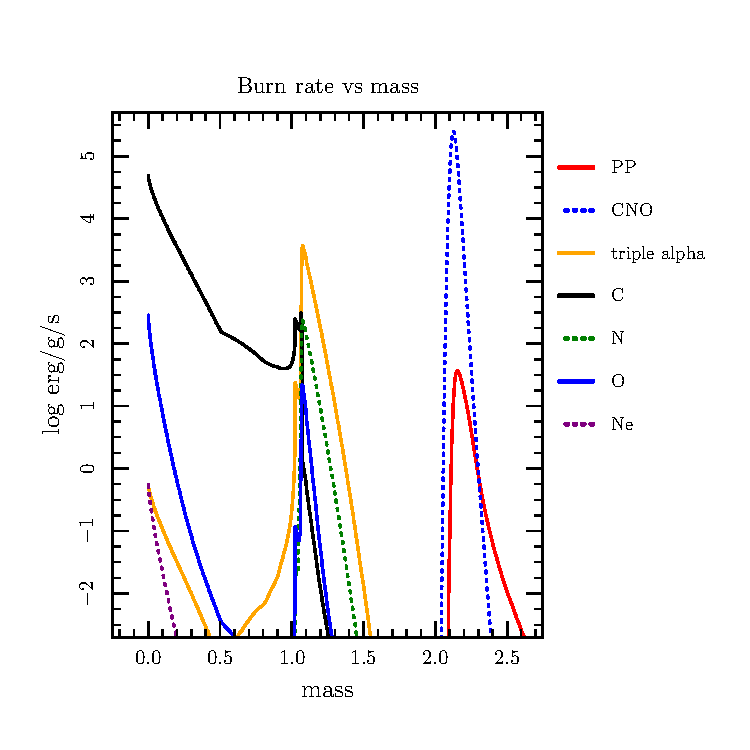
\includegraphics[width = 3.8in]{/Users/jaredbrooks/7M_prems_to_AGB/plots_out/Burnrate_vs_mass_52.pdf}
            \caption{Burning rate profile at orange dot}
            \label{fig:9}
          \end{minipage}
        \end{figure}

        \pagebreak

        To the left is a plot of the evolution of the center temperature and density (figure \ref{fig:10}).  To the right is a burning rate profile from the end of the run (figure \ref{fig:11}).

        \begin{figure}[H]
          \begin{minipage}[b]{0.5\linewidth}
            \centering
            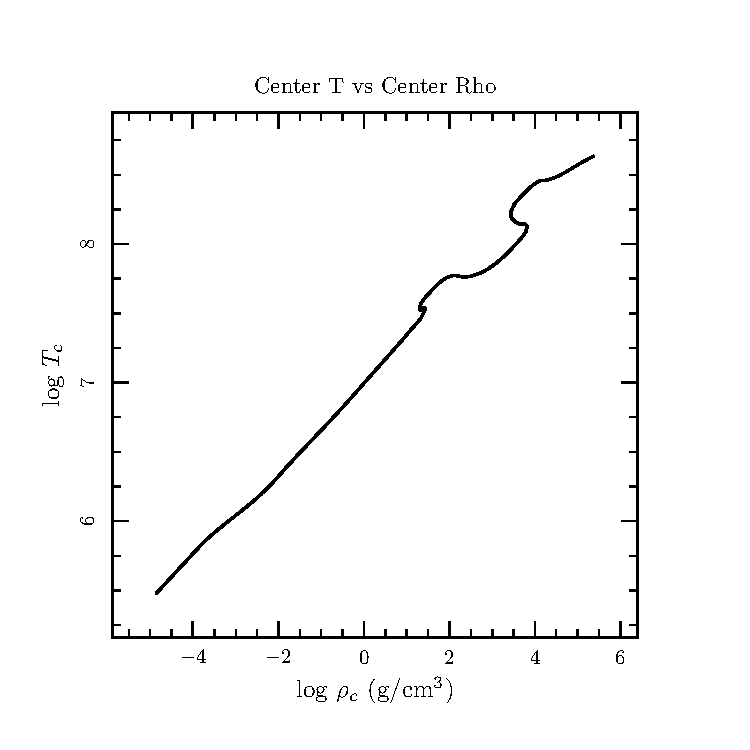
\includegraphics[width = 3.8in]{/Users/jaredbrooks/7M_prems_to_AGB/plots_out/Tc_vs_Rhoc.pdf}
            \caption{Evolution of center temperature and density}
            \label{fig:10}
          \end{minipage}
          \hspace{0cm}
          \begin{minipage}[b]{0.5\linewidth}
            \centering
            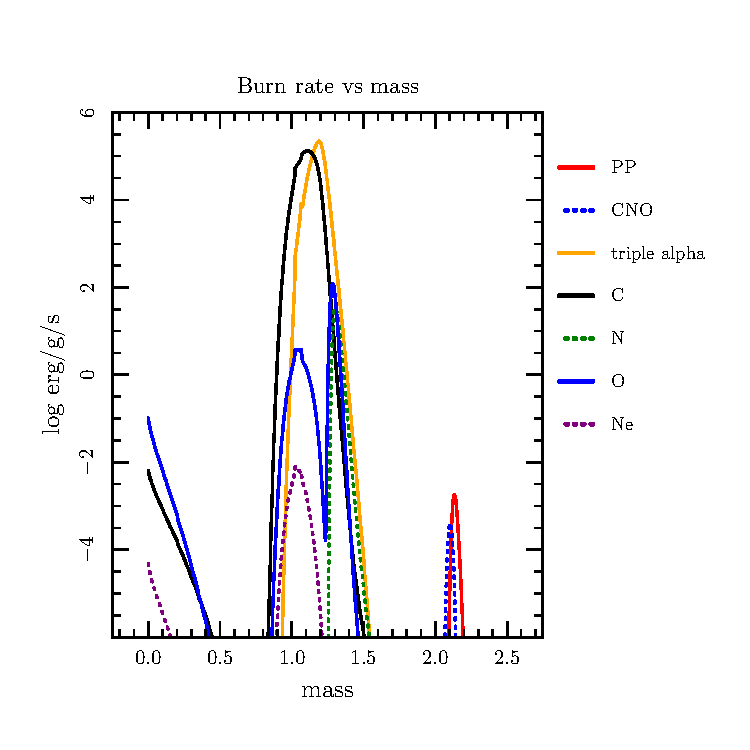
\includegraphics[width = 3.8in]{/Users/jaredbrooks/7M_prems_to_AGB/plots_out/Burnrate_vs_mass_59.pdf}
            \caption{Burning rate profile from end of run}
            \label{fig:11}
          \end{minipage}
        \end{figure}

        \pagebreak

        This final plot (figure \ref{fig:12}) shows a few internal \texttt{MESA} variables, such as the size of the time-step, the number of zones, and the number of retries against the model number in order to give some understanding of how hard \texttt{MESA} is working throughout the run and where some areas of problems/interest might be.

        \begin{figure}[H]
          \centering
          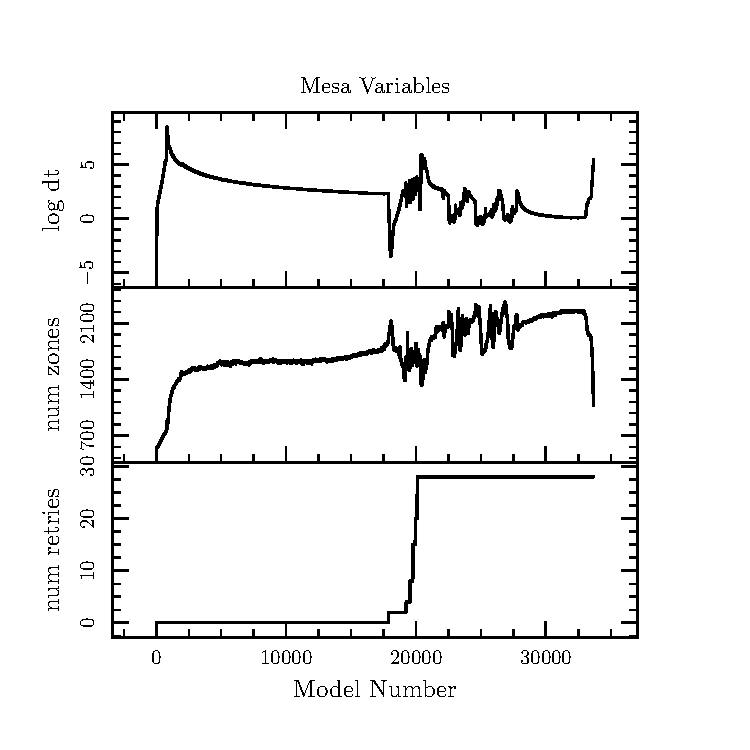
\includegraphics[width = 5in]{/Users/jaredbrooks/7M_prems_to_AGB/plots_out/Mesa_Variables.pdf}
          \caption{\texttt{MESA} variables plotted against model number show how hard \texttt{MESA} is working}
          \label{fig:12}
        \end{figure}


\end{document}
